
%% bare_jrnl.tex
%% V1.3
%% 2007/01/11
%% by Michael Shell
%% see http://www.michaelshell.org/
%% for current contact information.
%%
%% This is a skeleton file demonstrating the use of IEEEtran.cls
%% (requires IEEEtran.cls version 1.7 or later) with an IEEE journal paper.
%%
%% Support sites:
%% http://www.michaelshell.org/tex/ieeetran/
%% http://www.ctan.org/tex-archive/macros/latex/contrib/IEEEtran/
%% and
%% http://www.ieee.org/



% *** Authors should verify (and, if needed, correct) their LaTeX system  ***
% *** with the testflow diagnostic prior to trusting their LaTeX platform ***
% *** with production work. IEEE's font choices can trigger bugs that do  ***
% *** not appear when using other class files.                            ***
% The testflow support page is at:
% http://www.michaelshell.org/tex/testflow/


%%*************************************************************************
%% Legal Notice:
%% This code is offered as-is without any warranty either expressed or
%% implied; without even the implied warranty of MERCHANTABILITY or
%% FITNESS FOR A PARTICULAR PURPOSE! 
%% User assumes all risk.
%% In no event shall IEEE or any contributor to this code be liable for
%% any damages or losses, including, but not limited to, incidental,
%% consequential, or any other damages, resulting from the use or misuse
%% of any information contained here.
%%
%% All comments are the opinions of their respective authors and are not
%% necessarily endorsed by the IEEE.
%%
%% This work is distributed under the LaTeX Project Public License (LPPL)
%% ( http://www.latex-project.org/ ) version 1.3, and may be freely used,
%% distributed and modified. A copy of the LPPL, version 1.3, is included
%% in the base LaTeX documentation of all distributions of LaTeX released
%% 2003/12/01 or later.
%% Retain all contribution notices and credits.
%% ** Modified files should be clearly indicated as such, including  **
%% ** renaming them and changing author support contact information. **
%%
%% File list of work: IEEEtran.cls, IEEEtran_HOWTO.pdf, bare_adv.tex,
%%                    bare_conf.tex, bare_jrnl.tex, bare_jrnl_compsoc.tex
%%*************************************************************************

% Note that the a4paper option is mainly intended so that authors in
% countries using A4 can easily print to A4 and see how their papers will
% look in print - the typesetting of the document will not typically be
% affected with changes in paper size (but the bottom and side margins will).
% Use the testflow package mentioned above to verify correct handling of
% both paper sizes by the user's LaTeX system.
%
% Also note that the "draftcls" or "draftclsnofoot", not "draft", option
% should be used if it is desired that the figures are to be displayed in
% draft mode.
%
\documentclass[journal]{IEEEtran}
%
% If IEEEtran.cls has not been installed into the LaTeX system files,
% manually specify the path to it like:
% \documentclass[journal]{../sty/IEEEtran}





% Some very useful LaTeX packages include:
% (uncomment the ones you want to load)


% *** MISC UTILITY PACKAGES ***
%
%\usepackage{ifpdf}
% Heiko Oberdiek's ifpdf.sty is very useful if you need conditional
% compilation based on whether the output is pdf or dvi.
% usage:
% \ifpdf
%   % pdf code
% \else
%   % dvi code
% \fi
% The latest version of ifpdf.sty can be obtained from:
% http://www.ctan.org/tex-archive/macros/latex/contrib/oberdiek/
% Also, note that IEEEtran.cls V1.7 and later provides a builtin
% \ifCLASSINFOpdf conditional that works the same way.
% When switching from latex to pdflatex and vice-versa, the compiler may
% have to be run twice to clear warning/error messages.






% *** CITATION PACKAGES ***
%
\usepackage{cite}
% cite.sty was written by Donald Arseneau
% V1.6 and later of IEEEtran pre-defines the format of the cite.sty package
% \cite{} output to follow that of IEEE. Loading the cite package will
% result in citation numbers being automatically sorted and properly
% "compressed/ranged". e.g., [1], [9], [2], [7], [5], [6] without using
% cite.sty will become [1], [2], [5]--[7], [9] using cite.sty. cite.sty's
% \cite will automatically add leading space, if needed. Use cite.sty's
% noadjust option (cite.sty V3.8 and later) if you want to turn this off.
% cite.sty is already installed on most LaTeX systems. Be sure and use
% version 4.0 (2003-05-27) and later if using hyperref.sty. cite.sty does
% not currently provide for hyperlinked citations.
% The latest version can be obtained at:
% http://www.ctan.org/tex-archive/macros/latex/contrib/cite/
% The documentation is contained in the cite.sty file itself.






% *** GRAPHICS RELATED PACKAGES ***
%
\ifCLASSINFOpdf
   \usepackage[pdftex]{graphicx}
  % declare the path(s) where your graphic files are
  % \graphicspath{{../pdf/}{../jpeg/}}
  % and their extensions so you won't have to specify these with
  % every instance of \includegraphics
  % \DeclareGraphicsExtensions{.pdf,.jpeg,.png}
\else
  % or other class option (dvipsone, dvipdf, if not using dvips). graphicx
  % will default to the driver specified in the system graphics.cfg if no
  % driver is specified.
  % \usepackage[dvips]{graphicx}
  % declare the path(s) where your graphic files are
  % \graphicspath{{../eps/}}
  % and their extensions so you won't have to specify these with
  % every instance of \includegraphics
  % \DeclareGraphicsExtensions{.eps}
\fi
% graphicx was written by David Carlisle and Sebastian Rahtz. It is
% required if you want graphics, photos, etc. graphicx.sty is already
% installed on most LaTeX systems. The latest version and documentation can
% be obtained at: 
% http://www.ctan.org/tex-archive/macros/latex/required/graphics/
% Another good source of documentation is "Using Imported Graphics in
% LaTeX2e" by Keith Reckdahl which can be found as epslatex.ps or
% epslatex.pdf at: http://www.ctan.org/tex-archive/info/
%
% latex, and pdflatex in dvi mode, support graphics in encapsulated
% postscript (.eps) format. pdflatex in pdf mode supports graphics
% in .pdf, .jpeg, .png and .mps (metapost) formats. Users should ensure
% that all non-photo figures use a vector format (.eps, .pdf, .mps) and
% not a bitmapped formats (.jpeg, .png). IEEE frowns on bitmapped formats
% which can result in "jaggedy"/blurry rendering of lines and letters as
% well as large increases in file sizes.
%
% You can find documentation about the pdfTeX application at:
% http://www.tug.org/applications/pdftex





% *** MATH PACKAGES ***
%
%\usepackage[cmex10]{amsmath}
% A popular package from the American Mathematical Society that provides
% many useful and powerful commands for dealing with mathematics. If using
% it, be sure to load this package with the cmex10 option to ensure that
% only type 1 fonts will utilized at all point sizes. Without this option,
% it is possible that some math symbols, particularly those within
% footnotes, will be rendered in bitmap form which will result in a
% document that can not be IEEE Xplore compliant!
%
% Also, note that the amsmath package sets \interdisplaylinepenalty to 10000
% thus preventing page breaks from occurring within multiline equations. Use:
%\interdisplaylinepenalty=2500
% after loading amsmath to restore such page breaks as IEEEtran.cls normally
% does. amsmath.sty is already installed on most LaTeX systems. The latest
% version and documentation can be obtained at:
% http://www.ctan.org/tex-archive/macros/latex/required/amslatex/math/


\usepackage[utf8]{inputenc}
\usepackage[spanish]{babel}
\usepackage{float}
\usepackage{listings}
\usepackage{hyperref}

% *** SPECIALIZED LIST PACKAGES ***
%
%\usepackage{algorithmic}
% algorithmic.sty was written by Peter Williams and Rogerio Brito.
% This package provides an algorithmic environment fo describing algorithms.
% You can use the algorithmic environment in-text or within a figure
% environment to provide for a floating algorithm. Do NOT use the algorithm
% floating environment provided by algorithm.sty (by the same authors) or
% algorithm2e.sty (by Christophe Fiorio) as IEEE does not use dedicated
% algorithm float types and packages that provide these will not provide
% correct IEEE style captions. The latest version and documentation of
% algorithmic.sty can be obtained at:
% http://www.ctan.org/tex-archive/macros/latex/contrib/algorithms/
% There is also a support site at:
% http://algorithms.berlios.de/index.html
% Also of interest may be the (relatively newer and more customizable)
% algorithmicx.sty package by Szasz Janos:
% http://www.ctan.org/tex-archive/macros/latex/contrib/algorithmicx/




% *** ALIGNMENT PACKAGES ***
%
\usepackage{array}
% Frank Mittelbach's and David Carlisle's array.sty patches and improves
% the standard LaTeX2e array and tabular environments to provide better
% appearance and additional user controls. As the default LaTeX2e table
% generation code is lacking to the point of almost being broken with
% respect to the quality of the end results, all users are strongly
% advised to use an enhanced (at the very least that provided by array.sty)
% set of table tools. array.sty is already installed on most systems. The
% latest version and documentation can be obtained at:
% http://www.ctan.org/tex-archive/macros/latex/required/tools/


%\usepackage{mdwmath}
%\usepackage{mdwtab}
% Also highly recommended is Mark Wooding's extremely powerful MDW tools,
% especially mdwmath.sty and mdwtab.sty which are used to format equations
% and tables, respectively. The MDWtools set is already installed on most
% LaTeX systems. The lastest version and documentation is available at:
% http://www.ctan.org/tex-archive/macros/latex/contrib/mdwtools/


% IEEEtran contains the IEEEeqnarray family of commands that can be used to
% generate multiline equations as well as matrices, tables, etc., of high
% quality.


%\usepackage{eqparbox}
% Also of notable interest is Scott Pakin's eqparbox package for creating
% (automatically sized) equal width boxes - aka "natural width parboxes".
% Available at:
% http://www.ctan.org/tex-archive/macros/latex/contrib/eqparbox/





% *** SUBFIGURE PACKAGES ***
\usepackage[tight,footnotesize]{subfigure}
% subfigure.sty was written by Steven Douglas Cochran. This package makes it
% easy to put subfigures in your figures. e.g., "Figure 1a and 1b". For IEEE
% work, it is a good idea to load it with the tight package option to reduce
% the amount of white space around the subfigures. subfigure.sty is already
% installed on most LaTeX systems. The latest version and documentation can
% be obtained at:
% http://www.ctan.org/tex-archive/obsolete/macros/latex/contrib/subfigure/
% subfigure.sty has been superceeded by subfig.sty.



%\usepackage[caption=false]{caption}
%\usepackage[font=footnotesize]{subfig}
% subfig.sty, also written by Steven Douglas Cochran, is the modern
% replacement for subfigure.sty. However, subfig.sty requires and
% automatically loads Axel Sommerfeldt's caption.sty which will override
% IEEEtran.cls handling of captions and this will result in nonIEEE style
% figure/table captions. To prevent this problem, be sure and preload
% caption.sty with its "caption=false" package option. This is will preserve
% IEEEtran.cls handing of captions. Version 1.3 (2005/06/28) and later 
% (recommended due to many improvements over 1.2) of subfig.sty supports
% the caption=false option directly:
%\usepackage[caption=false,font=footnotesize]{subfig}
%
% The latest version and documentation can be obtained at:
% http://www.ctan.org/tex-archive/macros/latex/contrib/subfig/
% The latest version and documentation of caption.sty can be obtained at:
% http://www.ctan.org/tex-archive/macros/latex/contrib/caption/




% *** FLOAT PACKAGES ***
%
%\usepackage{fixltx2e}
% fixltx2e, the successor to the earlier fix2col.sty, was written by
% Frank Mittelbach and David Carlisle. This package corrects a few problems
% in the LaTeX2e kernel, the most notable of which is that in current
% LaTeX2e releases, the ordering of single and double column floats is not
% guaranteed to be preserved. Thus, an unpatched LaTeX2e can allow a
% single column figure to be placed prior to an earlier double column
% figure. The latest version and documentation can be found at:
% http://www.ctan.org/tex-archive/macros/latex/base/



%\usepackage{stfloats}
% stfloats.sty was written by Sigitas Tolusis. This package gives LaTeX2e
% the ability to do double column floats at the bottom of the page as well
% as the top. (e.g., "\begin{figure*}[!b]" is not normally possible in
% LaTeX2e). It also provides a command:
%\fnbelowfloat
% to enable the placement of footnotes below bottom floats (the standard
% LaTeX2e kernel puts them above bottom floats). This is an invasive package
% which rewrites many portions of the LaTeX2e float routines. It may not work
% with other packages that modify the LaTeX2e float routines. The latest
% version and documentation can be obtained at:
% http://www.ctan.org/tex-archive/macros/latex/contrib/sttools/
% Documentation is contained in the stfloats.sty comments as well as in the
% presfull.pdf file. Do not use the stfloats baselinefloat ability as IEEE
% does not allow \baselineskip to stretch. Authors submitting work to the
% IEEE should note that IEEE rarely uses double column equations and
% that authors should try to avoid such use. Do not be tempted to use the
% cuted.sty or midfloat.sty packages (also by Sigitas Tolusis) as IEEE does
% not format its papers in such ways.


%\ifCLASSOPTIONcaptionsoff
%  \usepackage[nomarkers]{endfloat}
% \let\MYoriglatexcaption\caption
% \renewcommand{\caption}[2][\relax]{\MYoriglatexcaption[#2]{#2}}
%\fi
% endfloat.sty was written by James Darrell McCauley and Jeff Goldberg.
% This package may be useful when used in conjunction with IEEEtran.cls'
% captionsoff option. Some IEEE journals/societies require that submissions
% have lists of figures/tables at the end of the paper and that
% figures/tables without any captions are placed on a page by themselves at
% the end of the document. If needed, the draftcls IEEEtran class option or
% \CLASSINPUTbaselinestretch interface can be used to increase the line
% spacing as well. Be sure and use the nomarkers option of endfloat to
% prevent endfloat from "marking" where the figures would have been placed
% in the text. The two hack lines of code above are a slight modification of
% that suggested by in the endfloat docs (section 8.3.1) to ensure that
% the full captions always appear in the list of figures/tables - even if
% the user used the short optional argument of \caption[]{}.
% IEEE papers do not typically make use of \caption[]'s optional argument,
% so this should not be an issue. A similar trick can be used to disable
% captions of packages such as subfig.sty that lack options to turn off
% the subcaptions:
% For subfig.sty:
% \let\MYorigsubfloat\subfloat
% \renewcommand{\subfloat}[2][\relax]{\MYorigsubfloat[]{#2}}
% For subfigure.sty:
% \let\MYorigsubfigure\subfigure
% \renewcommand{\subfigure}[2][\relax]{\MYorigsubfigure[]{#2}}
% However, the above trick will not work if both optional arguments of
% the \subfloat/subfig command are used. Furthermore, there needs to be a
% description of each subfigure *somewhere* and endfloat does not add
% subfigure captions to its list of figures. Thus, the best approach is to
% avoid the use of subfigure captions (many IEEE journals avoid them anyway)
% and instead reference/explain all the subfigures within the main caption.
% The latest version of endfloat.sty and its documentation can obtained at:
% http://www.ctan.org/tex-archive/macros/latex/contrib/endfloat/
%
% The IEEEtran \ifCLASSOPTIONcaptionsoff conditional can also be used
% later in the document, say, to conditionally put the References on a 
% page by themselves.





% *** PDF, URL AND HYPERLINK PACKAGES ***
%
%\usepackage{url}
% url.sty was written by Donald Arseneau. It provides better support for
% handling and breaking URLs. url.sty is already installed on most LaTeX
% systems. The latest version can be obtained at:
% http://www.ctan.org/tex-archive/macros/latex/contrib/misc/
% Read the url.sty source comments for usage information. Basically,
% \url{my_url_here}.





% *** Do not adjust lengths that control margins, column widths, etc. ***
% *** Do not use packages that alter fonts (such as pslatex).         ***
% There should be no need to do such things with IEEEtran.cls V1.6 and later.
% (Unless specifically asked to do so by the journal or conference you plan
% to submit to, of course. )


% correct bad hyphenation here
\hyphenation{op-tical net-works semi-conduc-tor}


\begin{document}
%
% paper title
% can use linebreaks \\ within to get better formatting as desired
\title{Honeynet para el análisis del tráfico y muestras de malware}
%
%
% author names and IEEE memberships
% note positions of commas and nonbreaking spaces ( ~ ) LaTeX will not break
% a structure at a ~ so this keeps an author's name from being broken across
% two lines.
% use \thanks{} to gain access to the first footnote area
% a separate \thanks must be used for each paragraph as LaTeX2e's \thanks
% was not built to handle multiple paragraphs
%

\author{Santiago de Diego,~\IEEEmembership{Estudiante UGR}
        Gustavo Romero,~\IEEEmembership{Profesor UGR}
\thanks{Santiago de Diego es estudiante del doble grado en matemáticas e ingeniería informática por la Universidad de Granada}% <-this % stops a space
\thanks{Gustavo Romero es profesor en la Universidad de Granada, en el departamento de Arquitectura y Tecnología de los Computadores}}

% note the % following the last \IEEEmembership and also \thanks - 
% these prevent an unwanted space from occurring between the last author name
% and the end of the author line. i.e., if you had this:
% 
% \author{....lastname \thanks{...} \thanks{...} }
%                     ^------------^------------^----Do not want these spaces!
%
% a space would be appended to the last name and could cause every name on that
% line to be shifted left slightly. This is one of those "LaTeX things". For
% instance, "\textbf{A} \textbf{B}" will typeset as "A B" not "AB". To get
% "AB" then you have to do: "\textbf{A}\textbf{B}"
% \thanks is no different in this regard, so shield the last } of each \thanks
% that ends a line with a % and do not let a space in before the next \thanks.
% Spaces after \IEEEmembership other than the last one are OK (and needed) as
% you are supposed to have spaces between the names. For what it is worth,
% this is a minor point as most people would not even notice if the said evil
% space somehow managed to creep in.



% The paper headers
\markboth{}%
{}
% The only time the second header will appear is for the odd numbered pages
% after the title page when using the twoside option.
% 
% *** Note that you probably will NOT want to include the author's ***
% *** name in the headers of peer review papers.                   ***
% You can use \ifCLASSOPTIONpeerreview for conditional compilation here if
% you desire.




% If you want to put a publisher's ID mark on the page you can do it like
% this:
%\IEEEpubid{0000--0000/00\$00.00~\copyright~2007 IEEE}
% Remember, if you use this you must call \IEEEpubidadjcol in the second
% column for its text to clear the IEEEpubid mark.



% use for special paper notices
%\IEEEspecialpapernotice{(Invited Paper)}




% make the title area
\maketitle


\begin{abstract}
%\boldmath
In this project we are about to deploy several honeypots in two Raspberry PI devices in order to analyze attacks directed to the UGR network. We present here a brief resume of the results of the experiment.
\\\\
On the one hand, we have results from a Kippo honeypot related to brute force attacks from several IP directions, most of them coming from Asia. In addition we show the results of a malware analysis of samples obtained from Kippo.
\\\\
On the other hand, we will obtain several results related to web attacks with another low/medium interaction honeypot, Glastopf.
\\\\
The purposes of this work are to identify and classify several samples of malware to show to the reader a general method to achieve this goal.
\end{abstract}
% IEEEtran.cls defaults to using nonbold math in the Abstract.
% This preserves the distinction between vectors and scalars. However,
% if the journal you are submitting to favors bold math in the abstract,
% then you can use LaTeX's standard command \boldmath at the very start
% of the abstract to achieve this. Many IEEE journals frown on math
% in the abstract anyway.

% Note that keywords are not normally used for peerreview papers.
\begin{IEEEkeywords}
Security, honeypots, honeynet, malware, traffic analysis
\end{IEEEkeywords}






% For peer review papers, you can put extra information on the cover
% page as needed:
% \ifCLASSOPTIONpeerreview
% \begin{center} \bfseries EDICS Category: 3-BBND \end{center}
% \fi
%
% For peerreview papers, this IEEEtran command inserts a page break and
% creates the second title. It will be ignored for other modes.
\IEEEpeerreviewmaketitle



\section{Introducción}
\IEEEPARstart{A}{ntes} del surgimiento de los honeypots, la seguridad era principalmente defensiva y se basaba en técnicas para parar a los atacantes. Existía mucha información sobre los elementos de un ataque tales como exploits, metodología del ataque… pero poca sobre los atacantes en sí. Por aquel entonces los administradores de sistemas no tenían ni tiempo ni los recursos necesarios para analizar todos los ataques. 
\\\\
En 1999 esto empezó a cambiar y se comenzó a estudiar también a los atacantes. Se desarrollaron los primeros dispositivos que se centraban en monitorizar los sistemas, lo que dio lugar al Honeypot Project. En algunos trabajos  (\cite{caracterizacion_atacantes} y \cite{caracterizacion_atacantes_2}) se emplea el uso de análisis de componentes principales para la caracterización de atacantes, mientras que otros (\cite{escala_atacantes}) se centran en elaborar una escala de clasificación de atacantes según su comportamiento.  Al principio los honeypots eran sistemas reales pero gracias a la virtualización, a lo largo de los años se fueron implementando soluciones más flexibles.
\\\\
Actualmente, constituyen una solución ampliamente utilizada para el análisis de los diversos factores que componen un ataque, por ejemplo algunos trabajos (\cite{practical_malware_analysis} y \cite{compiled_executables}) se centran en el análisis del malware, el primero de ellos proporciona un procedimiento genérico empleando análisis estático y dinámico para lidiar con esta problemática, del cual se han aplicado algunas nociones para realizar el presente trabajo. Otros como \cite{ofuscation} se centran en explicar las técnicas más comunmente empleadas para la ofuscación del malware, a fin de dificultar su desensamblado.
\\\\
Según su interacción con el usuario podemos clasificarlos en honeypots de \textbf{baja, media o alta interacción}. Los más interesantes de cara a la obtención de información son los últimos, pero también son los más complicados de gestionar.
\\\\
Podemos colocar un honeypot en tres posiciones distintas principalmente:
\begin{itemize}
\item\textbf{Detrás del firewall:} en esta posición se encuentra protegido por las reglas de filtrado del firewall y por tanto deberemos configurar este para que no bloquee ataques del exterior. Tiene la ventaja de que permite detectar ataques internos, además de la posibilidad de comprometer la red interna.
\item \textbf{Delante del firewall:} en esta posición se encuentra expuesto directamente a internet por lo que no es necesario configurar el firewall. Por contra, tiene la desventaja de que no permite detectar ataques internos.
\item \textbf{En una zona desmilitarizada:} el honeypot se encuentra en una zona donde se encuentran los servidores pero separada de la red interna. De esta forma permite recibir ataques tanto internos como externos sin comprometer la red interna. Tiene la desventaja de que será necesario también configurar el firewall.
\end{itemize}
\section{Escenario}
En este trabajo se han desplegado dos honepots de baja/media interacción, Kippo y Glastopf, en una posición delante del firewall a fin de poder recibir ataques procedentes del exterior. Para este propósito se han empleado dos dispositivos del tipo Raspberry Pi 3, uno de ellos con sistema operativo Raspbian y el otro con sistema operativo Honeeepi, una distribución especial que viene con varios honeypots preinstalados, lo cual facilita enormemente la labor de configuración. Se ha prestado especial atención a las medidas de seguridad de la honeynet a fin de no comprometer la red de la UGR, ya que al ser dispositivos vulnerables por definición y además el objetivo es que sean atacados, este punto es crucial.
\\\\
Para el análisis de las muestras de malware se han empleado máquinas virtuales con la misma arquitectura que el objetivo de las muestras, las cuales veremos en la sección correspondiente. Posteriormente, se ha procedido a la eliminación de dichas máquinas virtuales.
\section{Resultados obtenidos en el nodo Kippo}
En este momento se han recibido \textbf{29342} ataques dirigidos al puerto 22, todos ellos con patrones muy similares ,ver Fig. 1. La mayoría de ellos proceden de China, y en menor medida de Polonia, Vietnam y Holanda. Sin embargo, a pesar de la enorme tasa de ataques, resulta sorprendente la poca tasa de éxito de los mismos, ya que solamente el \textbf{12.62\%} de los mismos ha resultado existoso. Este dato resulta aún más sorprendente si tenemos en cuenta que se han empleado credenciales de acceso realmente sencillas (admin-admin, root-root…).
\begin{figure}[H]
\centerline{
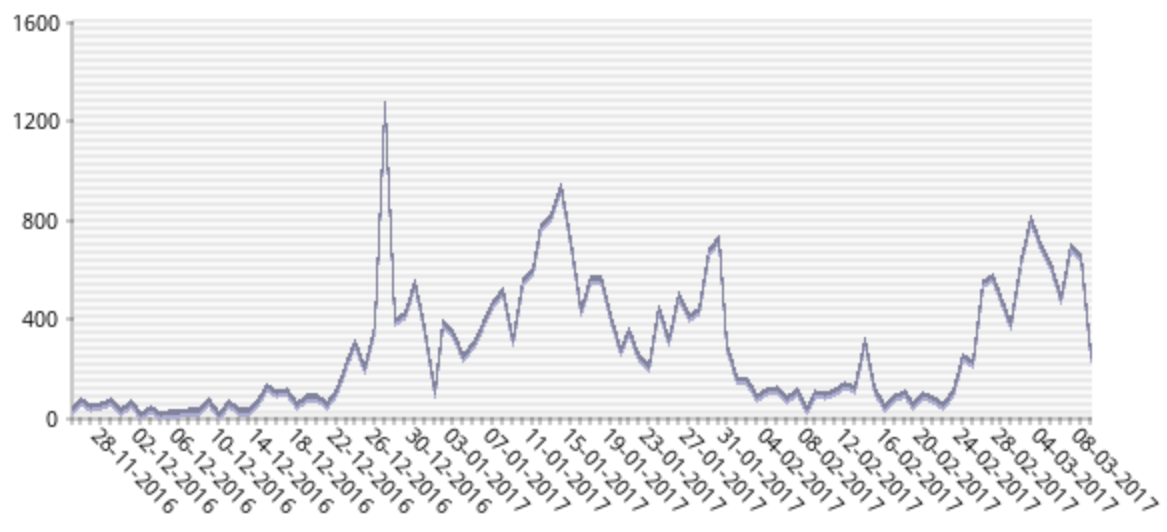
\includegraphics[width=9.5cm]{img/pruebas_dia}
}
\caption{Pruebas por día}
\label{fig:pruebas_diarias}
\end{figure}
En la imagen puede verse un incremento repentino cerca del 22 de Diciembre, que seguramente haya sido debido a que en esa fecha es cuando se terminó de ocultar el honeypot como tal, de forma que ya simulaba ser un servidor real. Además, al principio el servidor no era muy conocido pero en unas pocas semanas pudimos comprobar como apareció en el buscador \textit{Shodan} y por tanto era lógico esperar que el número de ataques recibidos se incrementase enormemente desde entonces.
\\\\
Por si fuera poco, se ha grabado las sesiones de los atacantes una vez entraban en el honeypot, a fin de poder descubrir patrones en su comportamiento. Por ejemplo, uno de los patrones observado es que todos ellos escribían a gran velocidad, así como que no cometían errores de escritura, por lo que es seguro que emplearon scripts automatizados para realizar los ataques. Podemos ver una de estas sesiones en la siguiente imagen:
\begin{figure}[H]
\centerline{
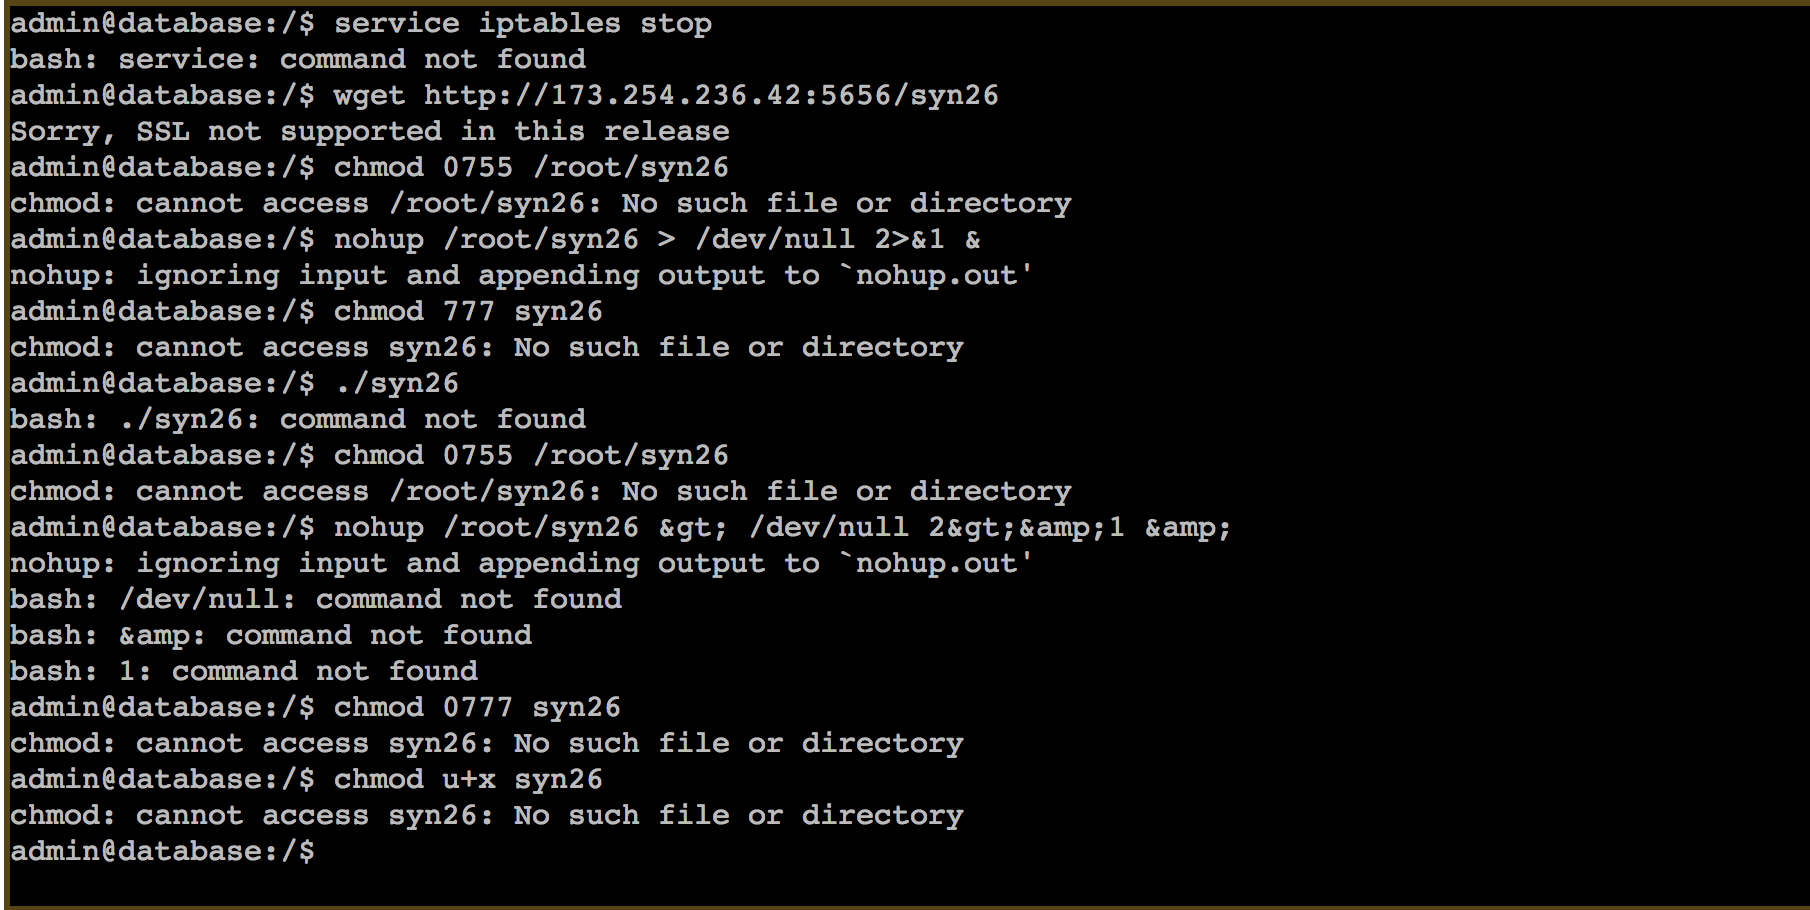
\includegraphics[width=9cm]{img/session}
}
\caption{Sesión grabada de un atacante}
\label{fig:sesion_atacante}
\end{figure}
Además hemos encontrado un patrón común a todos ellos:
\begin{enumerate}
\item El atacante accede al sistema por el puerto 22
\item Desactiva las reglas de filtrado del firewall
\item Descarga un fichero de una dirección IP remota
\item Ejecuta el fichero mediante el comando nohup, de forma que la ejecución continue cuando salga de la sesión
\end{enumerate}
A raíz del análisis de estos logs, se ha descubierto además que los atacantes siempre realizan acciones similares sin tener en cuenta la situación, por ejemplo, es común ver como un atacante intenta ejecutar un fichero que no ha sido descargado correctamente, o incongruencias similares (ver imagen anterior) y por tanto tenemos otro indicio de que los ataques son realmente automatizados.
\\\\
Además se ha procedido a clasificar a los atacantes por países, a fin de poder realizar estadísticas. Por ejemplo, podemos ver en la Fig. 3 una lista de los 10 países más beligerantes, de forma que se puede obtener una clasificación por países de los ataques recibidos.
\begin{figure}[H]
\centerline{
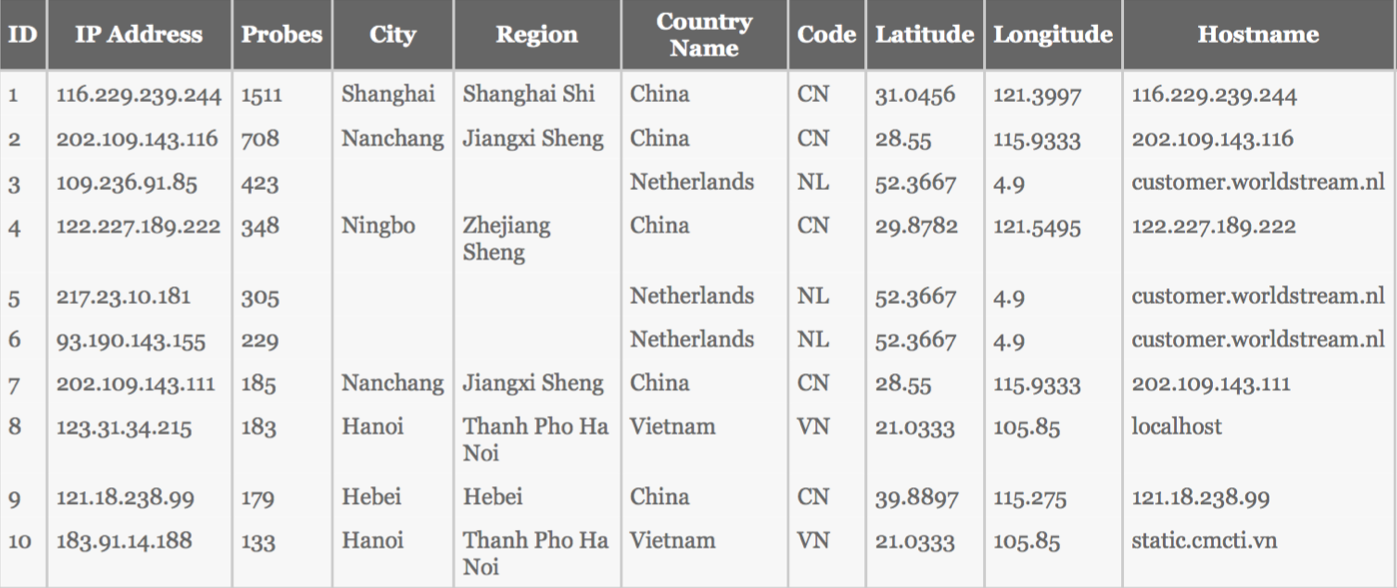
\includegraphics[width=8.8cm]{img/country_profiling}
}
\caption{Evaluación por paises}
\label{fig:sesion_atacante}
\end{figure}
Otra información útil puede ser ver qué clientes ssh han sido los más utilizados en los ataques, ya que esto puede ayudar a establecer clasificaciones de los diferentes atacantes según el tipo de máquina o sistema operativo que utilicen. Podemos ver también una clasificación de los 10 clientes más utilizados en la figura 4:
\begin{figure}[H]
\centerline{
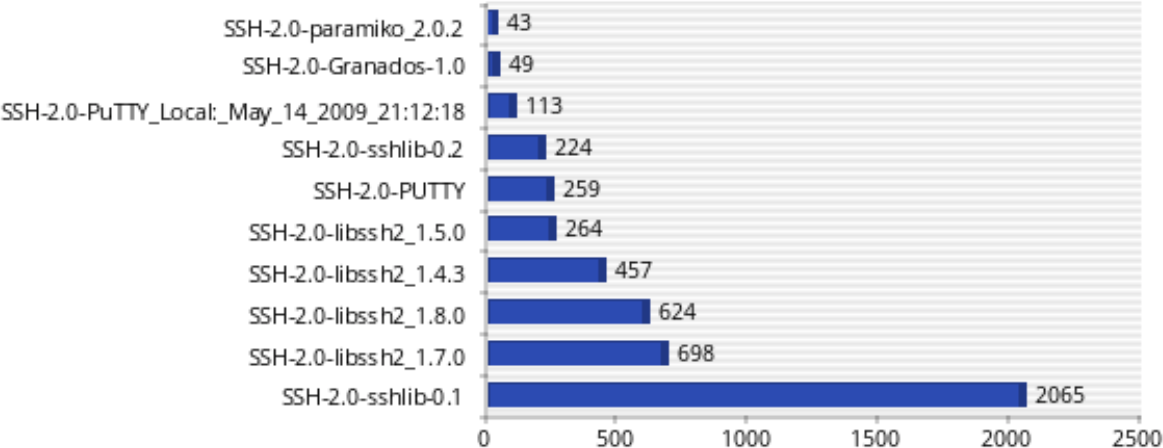
\includegraphics[width=8.8cm]{img/ssh}
}
\caption{Top 10 clientes ssh }
\label{fig:sesion_atacante}
\end{figure}
\section{Resultados obtenidos en el nodo Glastopf}
Centrándonos ahora en Glastopf, hemos recibido numerosos ataques del tipo inyección SQL, así como búsqueda de los ficheros \textit{robots.txt} o \textit{sitemap.xml}, ambos de ellos conocidos por contener información valiosa sobre la estructura de un sitio web. Además hemos encontrado varias pruebas hacia la ruta \textit{/wp-login.php}, debido a que el atacante ha debido creer que tenemos un \textit{wordpress} funcionando en el servidor y ha tratado de localizar el login.
\\\\
En otro ataque muy común, el atacante trata de acceder a la carpeta \textit{/shel}l, la cual no existe, lo que nos hace suponer que los ataques dirigidos al nodo Glastopf también son automatizados. El atacante escribe en dicha ubicación una cadena muy larga de caracteres, por ejemplo una como la siguiente (la más común):
\lstset{breaklines=true, alsoletter={\%}}
\begin{lstlisting}
/shell? %63 %64 %20 %2F %74 %6D %70 %3B %77 %67 %65 %74 %20 %68 %74 %74 %70 %3A %2F %2F %36 %31 %2E %31 %36 %30 %2E %32 %31 %33 %2E %32 %38 %3A %35 %34 %33 %32 %31 %2F %64 %6C %72 %2E %61 %72 %6D %3B %63 %68 %6D %6F %64 %20 %37 %37 %37 %20 %2A %3B %2E %2F %64 %6C %72 %2E %61 %72 %6D
\end{lstlisting}
la cual puede traducirse como:
\lstset{breaklines=true}
\begin{lstlisting}
cd /tmp &&
wget http://61.160.213.28:54321/dlr.arm;
chmod 777 *;./ dlr.arm
\end{lstlisting}
Se han encontrado varias cadenas de este tipo y todas ellas presentan un patrón similar:
\begin{enumerate}
\item El atacante se mueve a la carpeta /tmp ya que es el único lugar donde tiene permiso de escritura con el usuario www.
\item Descarga un binario malicioso de una dirección IP
\item Le asigna los permisos necesarios y lo ejecuta
\end{enumerate}
Además hemos observado que el origen de los ataques es, a diferencia de en Kippo, bastante diverso. Podemos encontrar ataques de países muy diferentes, como podemos observar en la figura 5. Se han empleado para el experimento 865 muestras, en lugar del enorme número de ataques registrados en Kippo. Esto es debido a que el ratio de ataques es mucho más bajo en el protocolo HTTP que en el SSH, debido a el tipo de explotación, ya que la segunda se presta más a su automatización por script kiddies1 que la primera.
\begin{figure}[H]
\centerline{
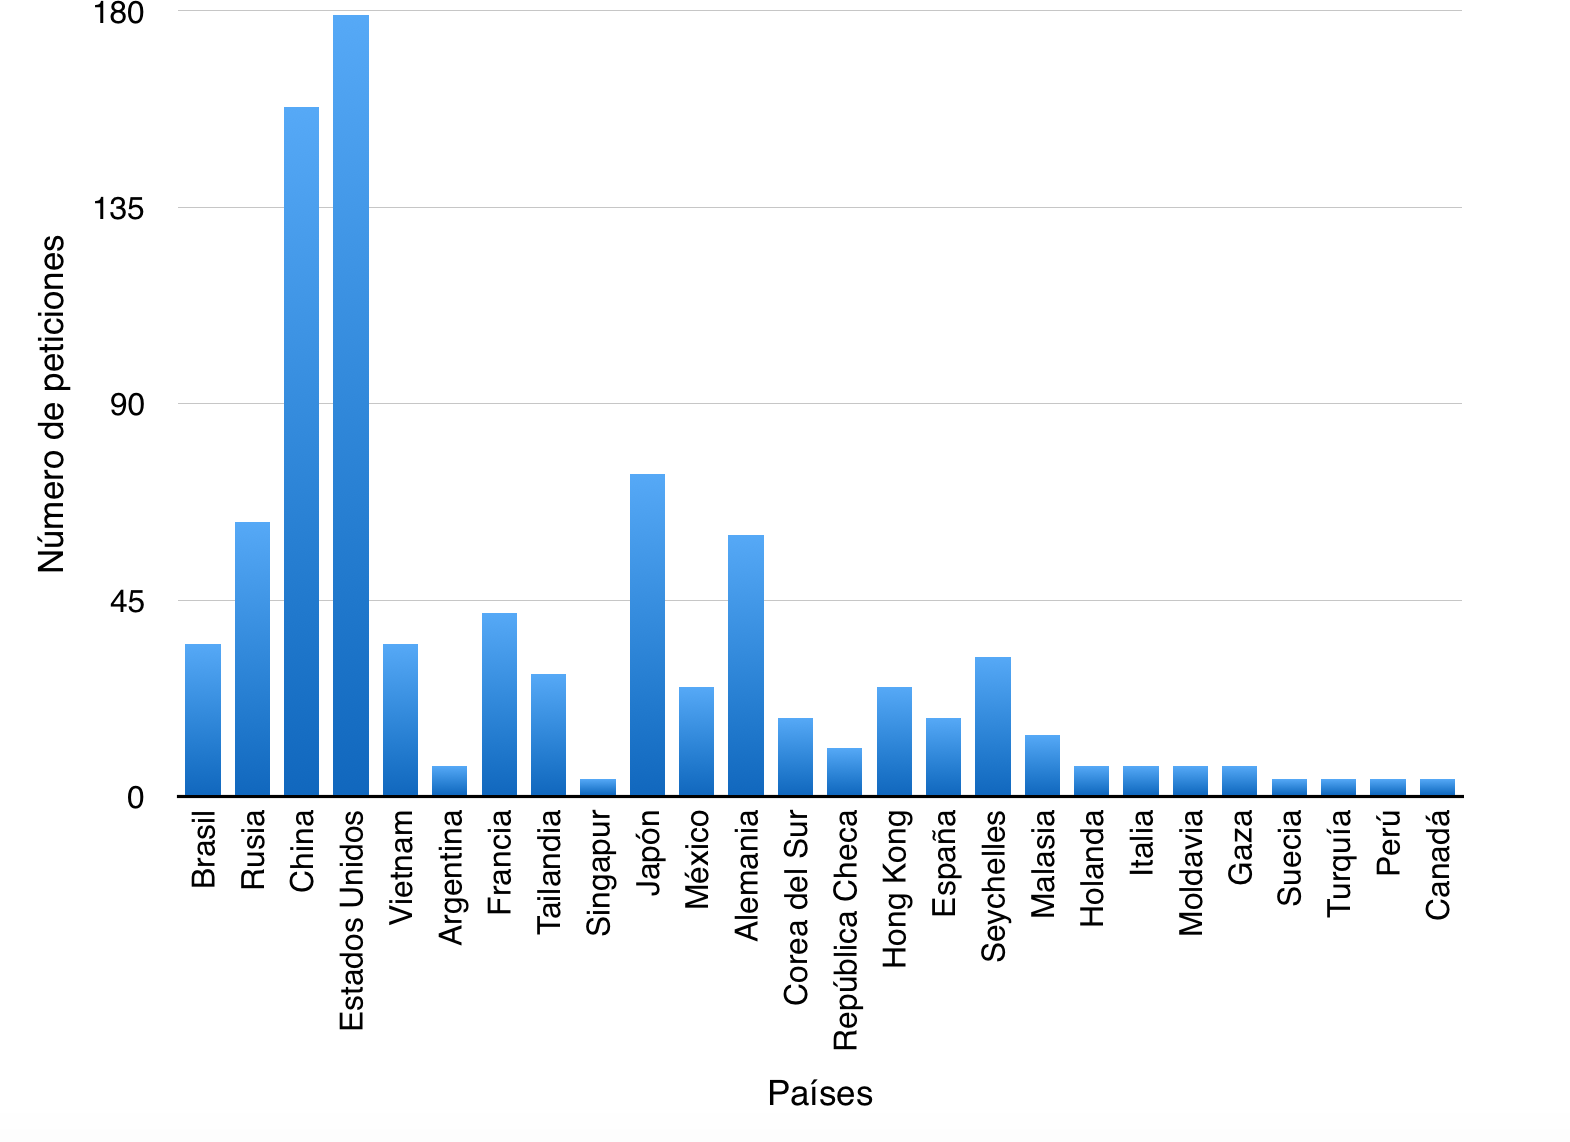
\includegraphics[width=8.8cm]{img/glastopf}
}
\caption{Número de ataques por día hacia Glastopf}
\label{fig:sesion_atacante}
\end{figure}
\section{Análisis de las muestras de malware obtenidas}
En esta sección analizaremos las diferentes muestras de malware que hemos obtenido mediante el nodo Kippo. Para tal fin se han empleado herramientas tanto manuales como automatizadas (objdump, gdb, radare, API de VirusTotal…).
\\\\
Las muestras recogidas son muy similares aunque con ligeras variaciones, como por ejemplo la IP a la que se conectan. La mayoría de ellas con binarios de tipo ELF~\footnote{Executable and Linkable Format}, están escritas en C/C++, para arquitectura x86 y su sistema operativo objetivo es Linux. La mayoría de ellas tienen como objetivo un procesador Intel 80386 Processor, pero algunas de ellas tienen como objetivo un MIPS R3000.
\\\\
Hemos descubierto que las muestras pertenecen a un tipo muy particular de malware chino, muy común y potencialmente dañino. Las muestras tienen funcionalidad de puerta trasera  y abren un puerto elegido aleatoriamente para conectarse a una IP remota. Además, se ha descubierto que son capaces de realizar ataques de denegación de servicio a otras máquinas una vez que han comprometido el host objetivo. Algo que nos ha llamado mucho la atención es que algunas muestras presentan información de depuración, por lo que nos hemos centrado en estas para poder obtener el máximo posible de información.
\\\\
Sospechamos que dichas muestras pueden pertenecer a la botnet \textit{BillGates}, calificada como de alto riesgo, a causa de las similitudes encontradas con otras muestras de malware de dicha botnet. Por ejemplo, un patrón en común es que todas ellas almacenan información en la librería \textit{/usr/libamplify.so} de sistemas Linux. Para realizar el análisis hemos empleado técnicas de ingeniería inversa, tales como el análisis estático y dinámico, todo ello en un entorno aislado y controlado. Si el lector quiere profundizar en estas tácticas de análisis, puede consultar \cite{know_your_enemy}, donde se proporcionan ejemplos y procedimientos para este fin.
\begin{figure}[H]
\centerline{
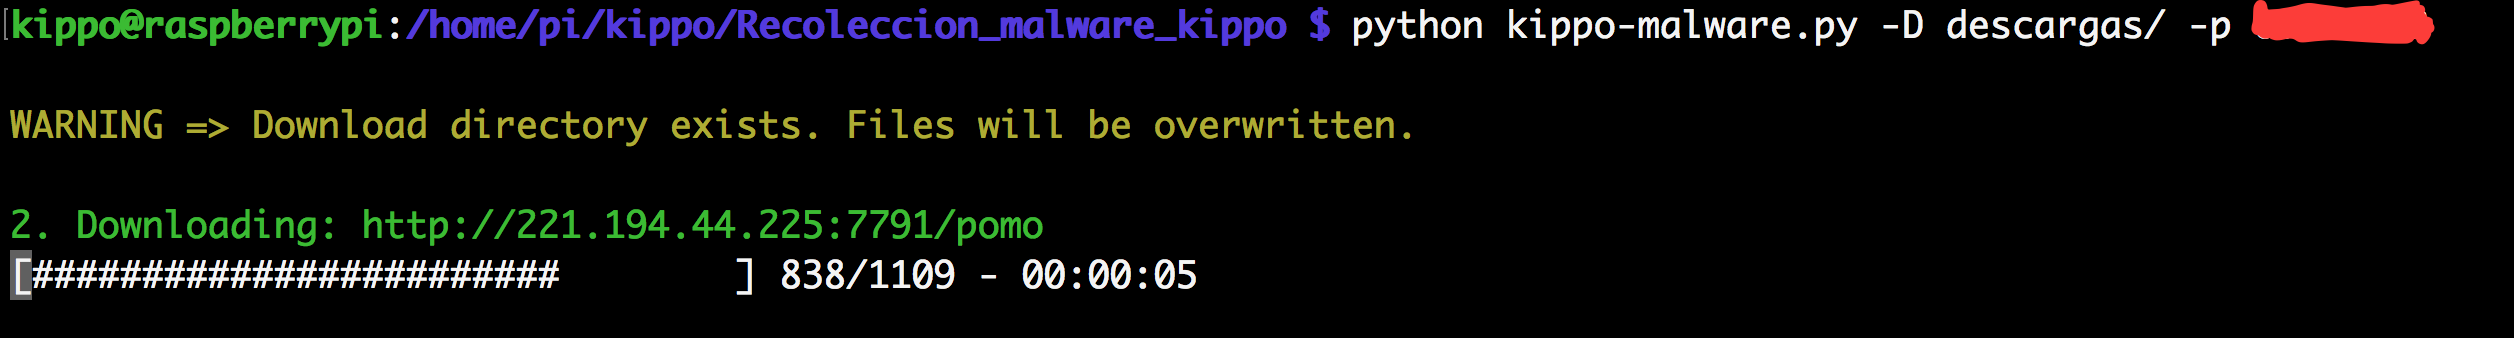
\includegraphics[width=8.8cm]{img/download_malware}
}
\caption{Descarga de malware desde uno de los honeypots}
\label{fig:sesion_atacante}
\end{figure}
Analizando la entropía de los binarios con radare hemos descubierto que no han sido encriptados, ya que dicha entropía es menor del \textbf{60\%}. Las muestras son bastante indetectables, ya que todas ellas fueron subidas a VirusTotal utilizando un script en Python y solamente cerca del \textbf{15\%} de los antivirus las detectaban como malware.
\\\\
Hemos descubierto varias funciones y variables que nos han permitido afianzar nuestras sospechas sobre el comportamiento del malware. Podemos ver una captura de las funciones de una de las muestras, extraídas con ddd en la Fig. 7:
\begin{figure}[H]
\centerline{
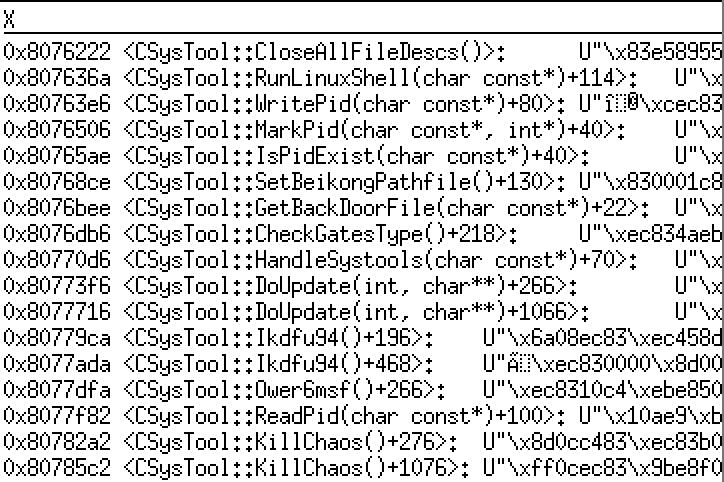
\includegraphics[width=8.5cm]{img/ddd}
}
\caption{Funciones empleadas por una de las muestras de malware}
\label{fig:sesion_atacante}
\end{figure}
Algunas herramientas de línea de comandos permiten recuperar este tipo de información por separado, como pueden ser file, strings o strace y pueden ser muy útiles para complementar la información obtenida examinando el código ensamblador. Un examen más exhaustivo del código, como mencionábamos anteriormente, revela funcionalidad de DOS. Podemos encontrar varias cadenas relacionadas con este tipo de ataque como son:
\begin{itemize}
\item \textit{AttackBase}
\item \textit{PacketAttack}
\item \textit{AttackUDP}
\item \textit{AttackSyn}
\item \textit{AttackICMP}
\item \textit{AttackDNS}
\item \textit{Tcpattack}
\end{itemize}
Un ejemplo de análisis dinámico corrobora que las muestras de malware son completamente funcionales y hacen lo que se espera de ellas. A modo de ejemplo, en la última línea de la imagen podemos ver la conexión con una ip desconocida:
\begin{figure}[H]
\centerline{
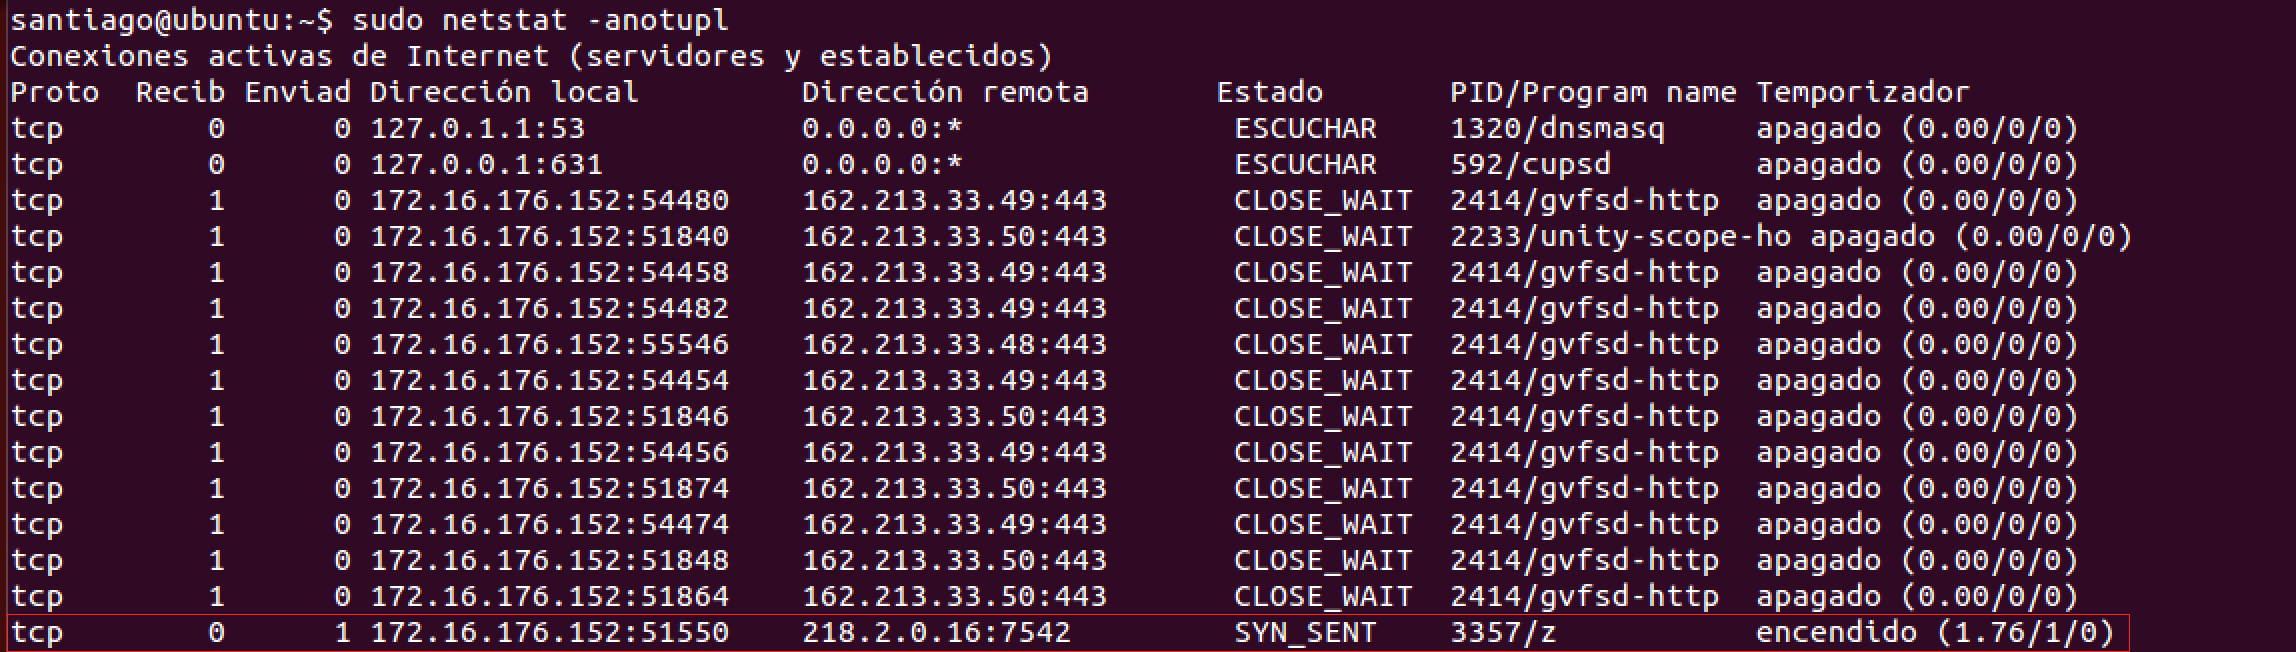
\includegraphics[width=8.9cm]{img/netstat}
}
\caption{Malware \textbf{z} conectándose con una IP remota}
\label{fig:sesion_atacante}
\end{figure}
\section{Conclusiones y trabajo futuro}
La principal conclusión que podemos extraer es que es esencial asegurar nuestros sistemas, ya que, aunque no somos conscientes, estamos recibiendo ataques constantemente. Además los atacantes disponen de mucho más tiempo y recursos que nosotros por lo que no debemos subestimarlos. Por tanto es imprescindible el sentido común para evitar ataques de ingeniería social, además de una sólida política de seguridad ya que, como hemos visto, la mayoría de los ataques son automatizados y pueden ser evitados. Enfatizamos en el empleo de contraseñas seguras y en evitar el uso de configuraciones “por defecto” para prevenir este tipo de ataques.
\\\\
Las futuras ampliaciones del trabajo, ordenadas por prioridad son:
\begin{enumerate}
\item Despliegue automático de la herramienta
\item Creación de una interfaz web que simplifique la configuración y el uso de la honeynet
\item Creación de nuevos nodos, con diferentes honeypots, algunos de ellos de alta interacción, a fin de obtener más información
\item Empleo de técnicas de clasificación automática usando técnicas de inteligencia artificial
\end{enumerate}
\section*{Agradecimientos}
Primero de todo, a mi tutor, Gustavo Romero del departamento de Arquitectura y  Tecnología de los Computadores, de la Universidad de Granada, por ayudarme en todo lo que ha podido y por recordarme conocimientos que había olvidado y han sido cruciales para el desarrollo de este proyecto. Por último pero no por ello menos importante, a mis padres por su constante apoyo y porque sin ellos nada de esto sería posible.
% Can use something like this to put references on a page
% by themselves when using endfloat and the captionsoff option.
\ifCLASSOPTIONcaptionsoff
  \newpage
\fi



% trigger a \newpage just before the given reference
% number - used to balance the columns on the last page
% adjust value as needed - may need to be readjusted if
% the document is modified later
%\IEEEtriggeratref{8}
% The "triggered" command can be changed if desired:
%\IEEEtriggercmd{\enlargethispage{-5in}}

% references section

% can use a bibliography generated by BibTeX as a .bbl file
% BibTeX documentation can be easily obtained at:
% http://www.ctan.org/tex-archive/biblio/bibtex/contrib/doc/
% The IEEEtran BibTeX style support page is at:
% http://www.michaelshell.org/tex/ieeetran/bibtex/
%\bibliographystyle{IEEEtran}
% argument is your BibTeX string definitions and bibliography database(s)
%\bibliography{IEEEabrv,../bib/paper}
%
% <OR> manually copy in the resultant .bbl file
% set second argument of \begin to the number of references
% (used to reserve space for the reference number labels box)
\begin{thebibliography}{1}

%\bibitem{IEEEhowto:kopka}
%H.~Kopka and P.~W. Daly, \emph{A Guide to \LaTeX}, 3rd~ed.\hskip 1em plus
  %0.5em minus 0.4em\relax Harlow, England: Addison-Wesley, 1999.

\bibitem{web_honeypot} Lukas Rist, Sven Vetsch, Marcel Koßin, Michael Maue,
\emph{A dynamic, low-interaction web application honeypot}. \hskip 1em plus
  0.5em minus 0.4em\relax The Honeynet Project, 2010. Disponible en: \url{https://www.honeynet.org/sites/default/files/files/KYT-Glastopf-Final_v1.pdf}

\bibitem{know_your_enemy} The honeypot project,
\emph{Know your enemy: learning about security threats}, 2nd~ed.\hskip 1em plus
  0.5em minus 0.4em
\relax Addison-Wesley, 2004 

\bibitem{virtual_honeypots} Niels Provos, Thorsten Holz,
\emph{Virtual Honeypots : from botnet tracking to intrusion detection}, 1st~ed.\hskip 1em plus
  0.5em minus 0.4em\relax Addison-Wesley, 2007.

\bibitem{clas_malware} Peter Kálnai, Jaromír Hořejší,
\emph{DDoS Trojan: A Malicious Concept that Conquered the ELF Format}. \hskip 1em plus
  0.5em minus 0.4em\relax Virus Bulletin, 2016. Disponible en: \url{https://www.virusbulletin.com/virusbulletin/2016/06/vb2015-paper-ddos-trojan-malicious-concept-conquered-elf-format/}

\bibitem{art_ampliacion} Mikhail Kuzinší,
\emph{Versatile DDoS Trojan for Linux}. \hskip 1em plus
  0.5em minus 0.4em\relax SecureList, 2014. Disponible en: \url{https://securelist.com/analysis/publications/64361/versatile-ddos-trojan-for-linux/}

\bibitem{art_botnet_billgates} Akamai’s Security Intelligence Research Team,
\emph{Threat Advisory: “BillGates” Botnet}.\hskip 1em plus
  0.5em minus 0.4em\relax Akamai’s [state of the internet] / security, 2016. Disponible en: \url{https://www.akamai.com/kr/ko/multimedia/documents/state-of-the-internet/bill-gates-botnet-threat-advisory.pdf}

\bibitem{ofuscation} Robbie Harwood and Maxime Serrano,
\emph{Lecture 26: Obfuscation}. \hskip 1em plus
  0.5em minus 0.4em\relax Carnegie Mellon University, 2013. Disponible en: \url{https://www.cs.cmu.edu/~fp/courses/15411-f13/lectures/26-obfuscation.pdf}

\bibitem{tracking_hackers} Lance Spitzner,
\emph{Honeypots: tracking hackers}, 1st~ed.\hskip 1em plus
  0.5em minus 0.4em
  \relax Addison-Wesley, 2002.

\bibitem{information_security} R.C. Joshi, Anjali Sardana,
\emph{Honeypots:A New Paradigm to Information Security}.\hskip 1em plus
  0.5em minus 0.4em
  \relax CRC Press, 2011


\bibitem{caracterizacion_atacantes} S. Almotairi, A. Clark, G. Mohay, and J. Zimmermann,
\emph{Characterization of Attackers’ Activities in Honeypot Traffic Using Principal Component Analysis}. \hskip 1em plus
  0.5em minus 0.4em
  \relax IFIP International Conference on Network and Parallel Computing, 2008.

\bibitem{caracterizacion_atacantes_2}S. Almotairi, A. Clark, G. Mohay, and J. Zimmermann,
\emph{A Technique for Detecting New Attacks in Low-Interaction Honeypot Traffic}. \hskip 1em plus
  0.5em minus 0.4em
  \relax  Fourth International Conference on Internet Monitoring and Protection, 2009

\bibitem{escala_atacantes}Gabriel Salles-Loustau, Robin Berthier, Etienne Collange, Bertrand Sobesto, and Michel Cukier,
\emph{Characterizing Attackers and Attacks: An Empirical Study}.\hskip 1em plus
  0.5em minus 0.4em
  \relax 17th IEEE Pacific Rim International Symposium on Dependable Computing, 2011.

\bibitem{practical_malware_analysis} Kris Kendall,
\emph{Practical malware analysis}. \hskip 1em plus
  0.5em minus 0.4em
  \relax 17th IEEE Pacific Rim International Symposium on Dependable Computing, 2011.
  
\bibitem{compiled_executables}Quist, Daniel A. Liebrock, Lorie M.,
\emph{Visualizing compiled executables for malware analysis}. \hskip 1em plus
  0.5em minus 0.4em
  \relax 6th International Workshop on Visualization for Cyber Security, 2009.

\end{thebibliography}


\end{document}


